\section{Evaluation}
To evaluate irpSSHa, two IP flow log datasets were used as input. The flow logs were collected from VPC Flow Logs monitoring on an AWS EC2 t1.micro instance running Ubuntu 14.04 in the US East (N. Virginia) region. The first input dataset spanned a time period of four days, from midnight GMT on January 8th, 2018, to midnight GMT on January 12th, 2018. The second spanned a time period of four hours, from 1:00am GMT on January 15th, 2018, to 5:00am GMT on January 15th, 2018. The datasets included 13058 and 476 flow records, respectively. The irpSSHa output for each can be seen in Figure~\ref{fig:output1} and Figure~\ref{fig:output2}

\begin{figure}[h]
%\resizebox{\textwidth}{!}
{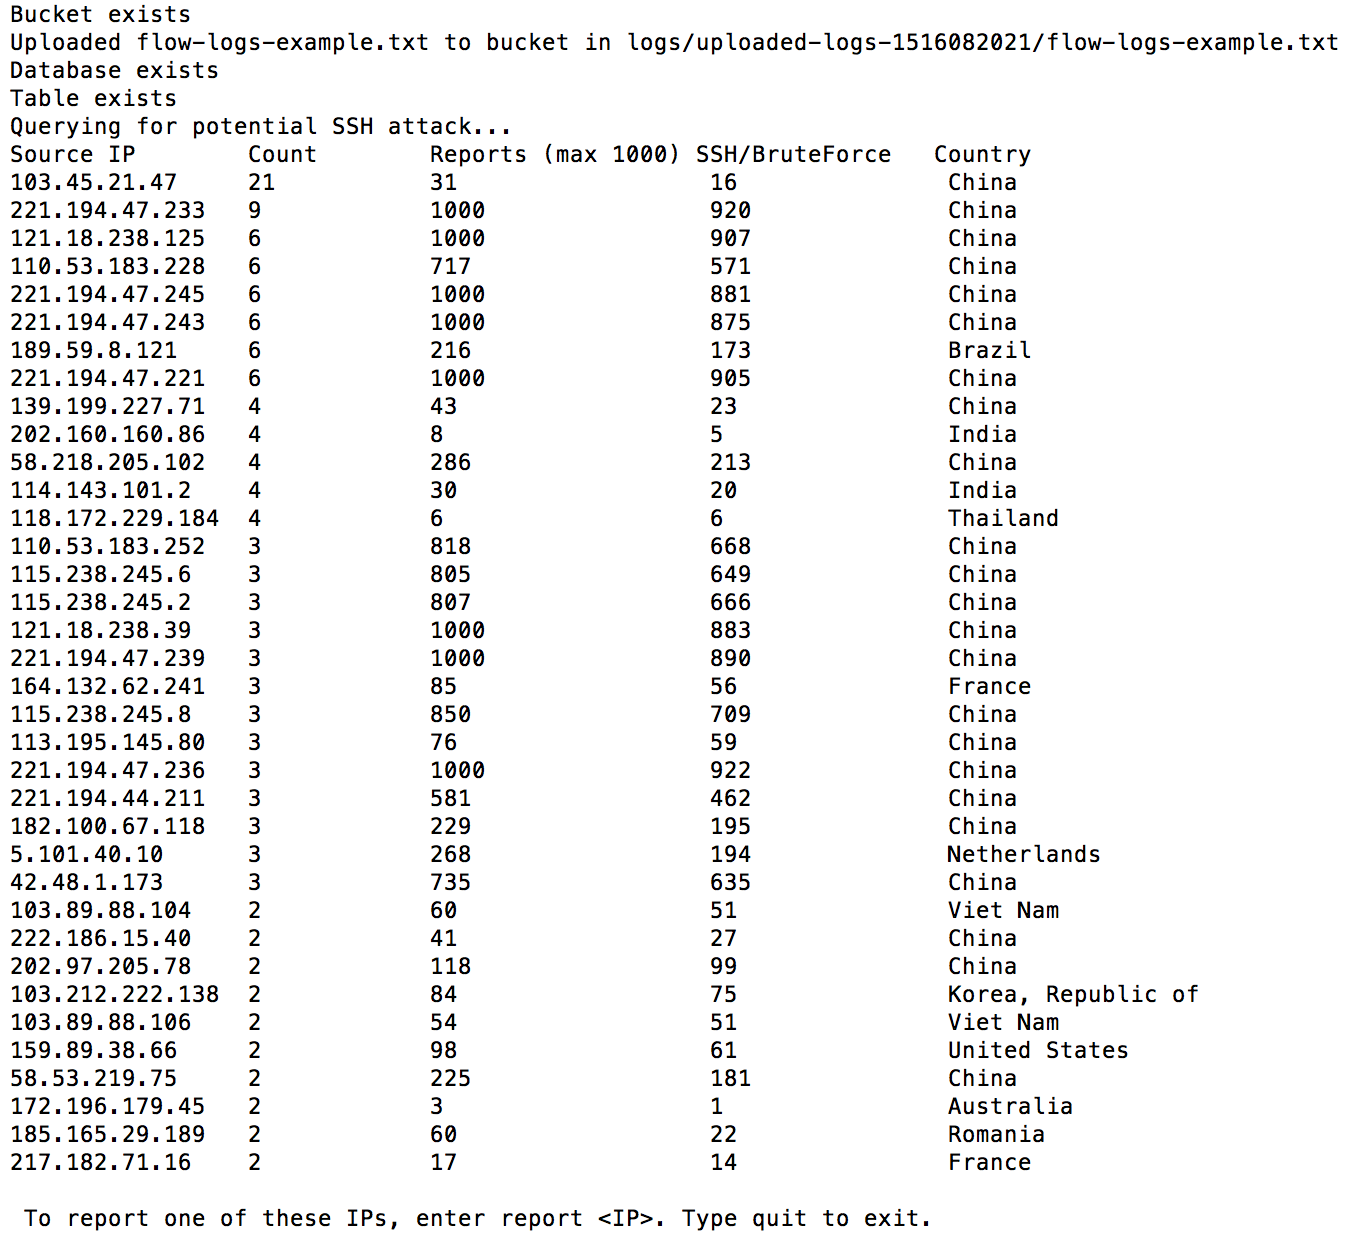
\includegraphics[width=3in]{./figures/561-irpSSHa-output-1.png}}
%{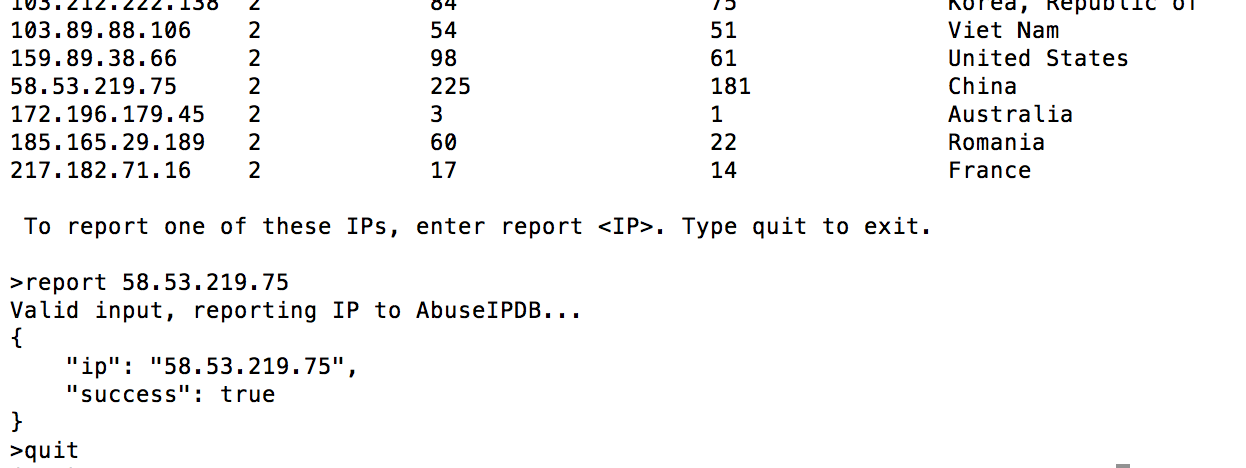
\includegraphics{./figures/561-irpSSHa-prompt.png}}
\caption{\small{Output from running irpSSHa with the first example IP flow dataset}}
\label{fig:output1}
\end{figure}

\begin{figure}[h]
%\resizebox{\textwidth}{!}
{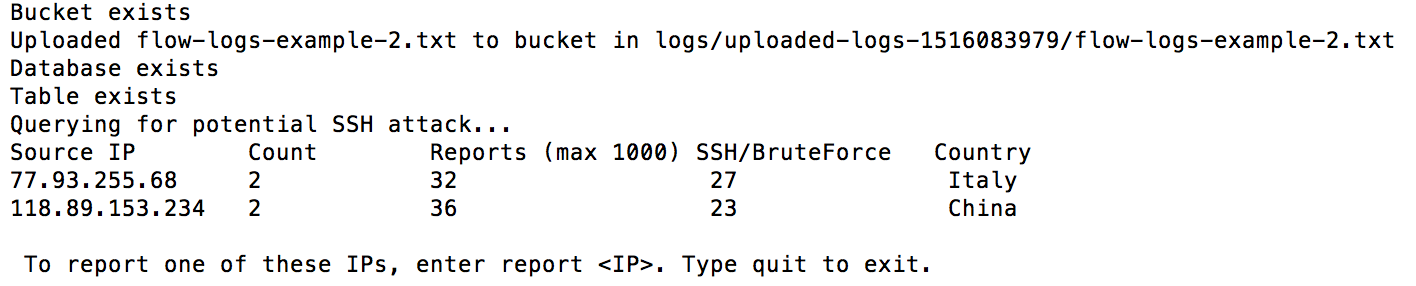
\includegraphics[width=3in]{./figures/561-irpSSHa-output-2.png}}
%{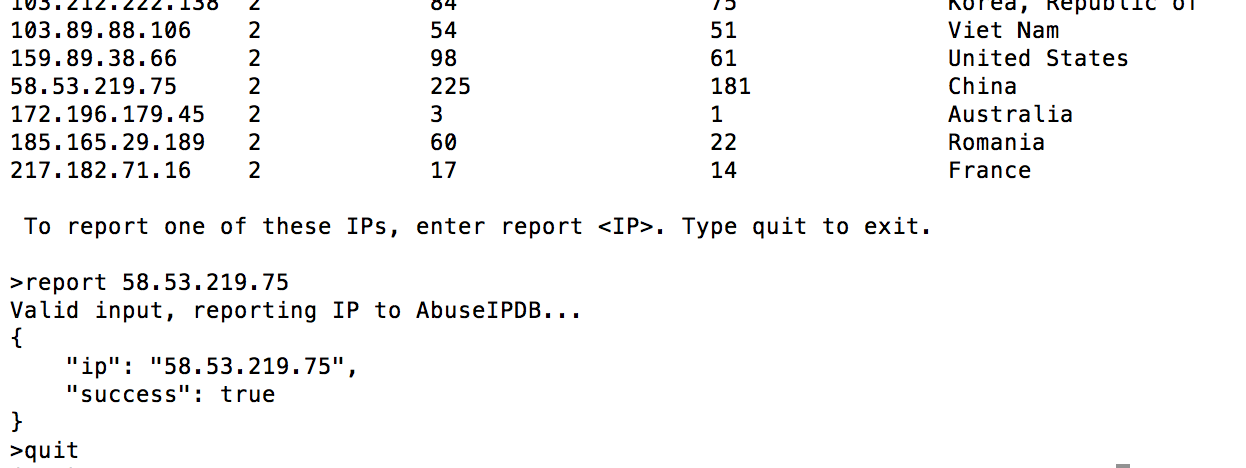
\includegraphics{./figures/561-irpSSHa-prompt.png}}
\caption{\small{Output from running irpSSHa with the second example IP flow dataset}}
\label{fig:output2}
\end{figure}

The output is separated into five columns. The Source IP column contains distinct IPs that were identified as potential SSH brute force attackers within the input flows. The Count column contains the number of flows in the input that contained unauthorized SSH access attempts from the IP. The Reports column indicates how many times in the past 60 days the source IP has been reported to AbuseIPDB. A limitation of the AbuseIPDB API is that the maximum value returned for this field is 1000, so source IPs with 1000 reports in the output were very likely reported a significant number of times \textit{more} than 1000. The data in the fourth column represents the number of these reports in AbuseIPDB that indicated the IP was suspected of an SSH attack, brute force attack, or both. The last column contains the name of the country in which the source IP originates.

As seen in the output, the smaller dataset indicated two IPs potentially involved in SSH brute force attack attempts. In both executions of irpSSHa, the minimum threshold for observing unauthorized SSH access attempts was two flows. Each IP in the smaller input's results was reported to AbuseIPDB at least 30 times within the last 60 days, with the majority of each implicating the IP in SSH and/or brute force attacks. The output for the larger dataset identifies 36 different source IPs as potential attackers, with 8 of them having been reported at least 1000 times within the last 60 days to AbuseIPDB. The potential attackers were responsible for a total of 145 unauthorized SSH access attempts (the sum of the Count column). If we decrease the minimum threshold from two to one, AbuseIPDB rate limits are quickly exceeded, but 101 more IPs are identified from the larger dataset, bringing the total up to 246 potential brute force attack attempts in four days. While not quite as large as some reports using dedicated honeypots, these numbers are consistent with what would be expected. In addition, we observe that, of the 36 source IPs in the larger input's table, 23 or about 64\% of them originate in China.
\label{sec:eval}

